%biblio : https://www.lirmm.fr/~wpuech/enseignement/master_informatique/Compression_Insertion/Dissimulation_de_donnees_Cours3.pdf
% https://histoiresecretes.wordpress.com/2013/05/05/la-steganographie-par-substitution/
% http://www.math.ucsd.edu/~crypto/Projects/MaxWeiss/steganography.pdf
\paragraph{Définition}~\\\indent
La stéganographie par substitution de \emph{LSB} (\emph{Least Significant Bit}) -- dans l'exemple de la stéganographie au travers d'une image -- consiste à substituer les bits de poids faibles (les \emph{LSB}) des pixels de l'image originale par les bits du message que l'on souhaite insérer. À la réception de l'image, le destinataire du message caché doit savoir au préalable dans quel sens parcourir les pixels pour retrouver le message (usuellement, parcours pseudo-aléatoire choisi, avec une clé secrète $k$).

\paragraph{Exemple}~\\\indent
\underline{Message ($M$) :} $M = 11001000$ ~\\\\\indent
\underline{Traitement de l'image en niveau de gris :} ~\\\indent
On découpe le message $M$=\textbf{\textcolor{red}{1}
						  \textcolor{blue}{1}
						  \textcolor{green}{0}
						  \textcolor{orange}{0}
						  \textcolor{gray}{1}
						  \textcolor{Brown}{0}
						  \textcolor{RubineRed}{0}
						  \textcolor{Violet}{0}}
 
 ~\\

\begin{minipage}{.5\textwidth}\centering
	\begin{tabular}{|c|c|c|c|}
	\hline
	00110100 & 11001010 & 01101001 & 11101101 \\\hline
	10000010 & 10100100 & 00101101 & 10111011 \\\hline
	\end{tabular}
	\captionof{table}{Image originale en niveaux de gris}
\end{minipage}
\begin{minipage}{.5\textwidth}\centering
	\begin{tabular}{|c|c|c|c|}
	\hline
	0011010\textcolor{red}{\textbf{1}} & 1100101\textcolor{blue}{\textbf{1}} & 0110100\textcolor{green}{\textbf{0}} & 1110110\textcolor{orange}{\textbf{0}} \\\hline
	1000001\textcolor{gray}{\textbf{1}} & 1010010\textcolor{Brown}{\textbf{0}} & 0010110\textcolor{RubineRed}{\textbf{0}} & 1011101\textcolor{Violet}{\textbf{0}} \\\hline
	\end{tabular}
	\captionof{table}{Image modifiée en niveaux de gris}
\end{minipage}

\paragraph{Application}~\\\indent
On utilise un programme \textsf{Matlab} permettant de réaliser de la stéganographie par substitution de \emph{LSB}. On fournit à ce programme deux images carrées de dimension similaires : l'une des images est la \emph{cover} (l'image dans laquelle on veut dissimuler un message), la seconde est l'image à cacher. Le programme transforme ensuite ces images en niveaux de gris. On choisit également le nombre de bits à substituer.\\

Voici un exemple d'application. La stéganographie est ici réalisée par substitution d'un seul bit : le bit de plus faible poids. 

\begin{minipage}{.5\textwidth}\centering
	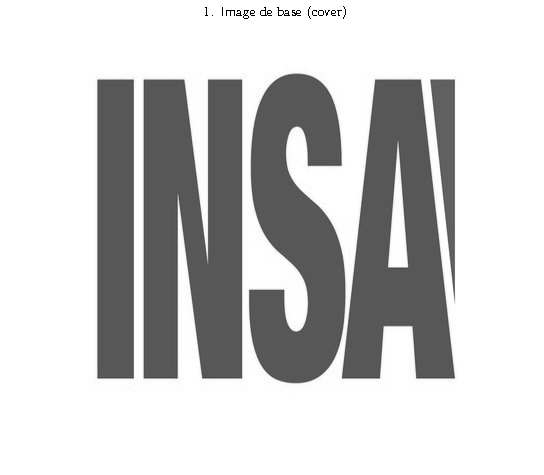
\includegraphics[scale=0.4]{images/fig1.png}
	\captionof{figure}{Image de base (\emph{cover})}
	\label{fig1}
\end{minipage}
\begin{minipage}{.5\textwidth}\centering
	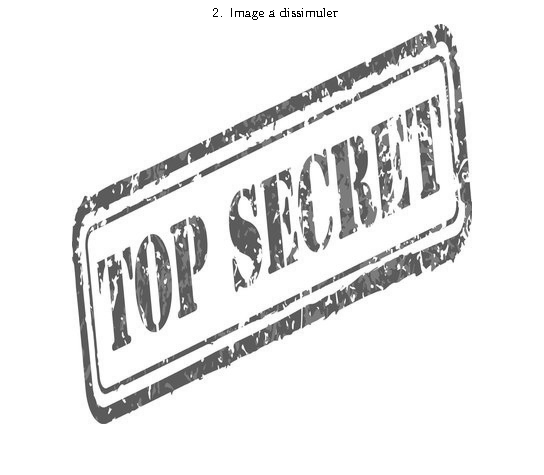
\includegraphics[scale=0.4]{images/fig2.png}
	\captionof{figure}{Image à dissimuler}
	\label{fig2}
\end{minipage}


\begin{minipage}{.5\textwidth}\centering
	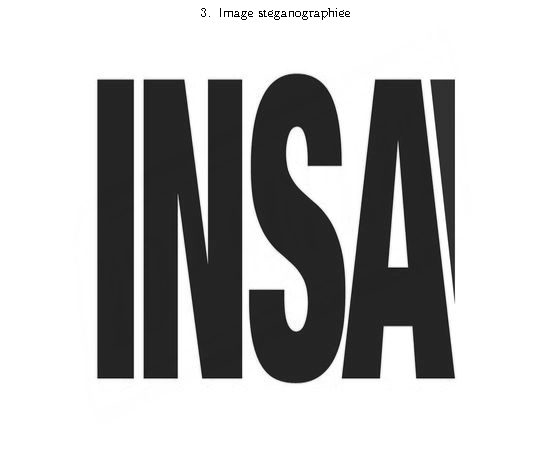
\includegraphics[scale=0.4]{images/fig3.png}
	\captionof{figure}{Image stéganographiée}
	\label{fig3}
\end{minipage}
\begin{minipage}{.5\textwidth}\centering
	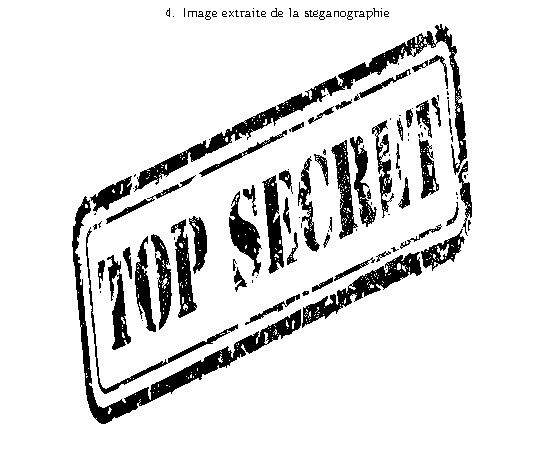
\includegraphics[scale=0.4]{images/fig4.png}
	\captionof{figure}{Image extraite de la stéganographie}
	\label{fig4}
\end{minipage}


\begin{minipage}{.5\textwidth}\centering
	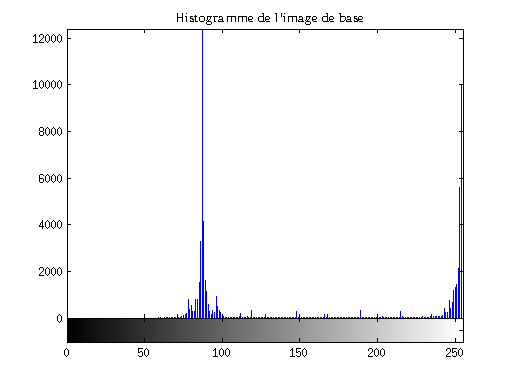
\includegraphics[scale=0.4]{images/fig5.png}
	\captionof{figure}{Histogramme de l'image \emph{cover}}
	\label{fig5}
\end{minipage}
\begin{minipage}{.5\textwidth}\centering
	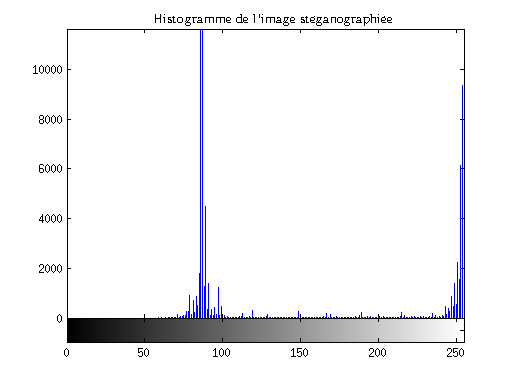
\includegraphics[scale=0.4]{images/fig6.png}
	\captionof{figure}{Histogramme de l'image stéganographiée}
	\label{fig6}
\end{minipage}

\paragraph{Commentaires}~\\\indent
Sur la figure \ref{fig3}, on ne voit pas à l'\oe il nu qu'un message est dissimulé. Pourtant, on voit bien sur la figure \ref{fig4} qu'un message caché a pu être extrait de l'image stéganographiée. Ce message caché est même récupéré sans trop de distorsion. Le programme nous renvoie les résultats suivants pour le PSNR\footnote{\emph{Peak Signal to Noise Ratio}.} et l'EQM\footnote{Erreur Quadratique Moyenne.} : 
$$ EQM = \frac{1}{m\cdot n}\sum_{i=0}^{m-1}\sum_{j=0}^{n-1}\big(I_1(i,j)-I_2(i,j) \big)^2 = 1.39\times 10^4$$
où $I_1$ représente l'image originale à dissimuler, $I_2$ est l'image dissimulée récupérée après la stéganographie, $m$ est la hauteur des images et $j$ est la largeur des images. L'EQM est relativement élevée puisqu'elle compare chaque pixel entre les deux images, et qu'ici les pixels sont modifiés, bien que très peu puisqu'on ne change que le bit de poids faible de certains des pixels, mais modifiés tout de même.
$$PSNR = 10\cdot \log_{10}\left(\frac{d^2}{EQM}\right) = 10.6027 $$
où $d$ est la dynamique du signal, donc ici la valeur maximale qu'un pixel peut avoir, soit $d=255$ dans notre cas (pixels codés sur 8 bits).

Enfin on voit sur les figures \ref{fig5} et \ref{fig6} que les histogrammes sont grossièrement identiques, ce qui est logique. En effet, seul le bit de plus faible poids est modifié ici. Ce bit est donc celui qui apporte le moins d'information sur chacun des pixels. Sa modification n'a donc pas un impact grave sur le pixel original.

\paragraph{Critique de cette méthode}
\begin{description}
\item[Avantage] Facile à implémenter et calculs de complexité relativement faible.
\item[Inconvénient] Assez facilement repérable et attaquable (attaque du $\chi^2$) car, bien que peu visible à l'\oe il nu, la distribution statistique du support est relativement altérée. 
\end{description}
